\section{字符串}
\begin{frame}[fragile]
  \frametitle{字符串}
  计算机非数值处理的对象经常是字符串数据。如信息检索、文本聚类、文本理解等。

  \begin{itemize}
  \item 串的定义及表示
  \item 串的模式匹配
  \end{itemize}
\end{frame}

\begin{frame}[fragile]
  \frametitle{串 (String)的定义}

  \begin{itemize}
  \item 串是由零个或多个任意字符组成的字符序列。它也是一种特殊的线性表,其数据元
    素仅由一个字符组成,而且它通常是作为一个整体来处理。

例:s="Renmin University",s是串名, Renmin University为串值,其中一个个的字符称
为串的元素。

  \item 请思考如何实现上述串的存储?
  \end{itemize}
\end{frame}

\begin{frame}[fragile]
  \frametitle{字符串的存储}
  \begin{itemize}
  \item 顺序存储: 用一组地址连续的存储单元存储串值中的字符序列。
  \item 链式存储: 考虑到存储密度,可以按块分配。
  \item 在Python/C/Java等语言中,String就是字符串。在C语言中没有string类型变量,字符串用字符数组表示。
  \end{itemize}
\end{frame}

\begin{frame}[fragile]
  \frametitle{串的模式匹配}
  \begin{itemize}
  \item 设s和t是给定的两个串,在主串s中寻找等于子串t的部分的过程称为模式匹配, t也称为模式。
  \item 如果在s中找到等于t的子串,则称匹配成功,返回t在s中的首次出现的存储位置,否则匹配失败。
  \item 例:

    s="ababcabcacbab"

    t="abcac"
  \end{itemize}
\end{frame}

\begin{frame}[fragile]
  \frametitle{简单的模式匹配}
  \begin{columns}
    \begin{column}[T]{0.5\linewidth}
      s="ababcabcacbab" \\ t="abcac"

      \begin{itemize}
      \item Brute-Force算法
      \end{itemize}
    \end{column}
    \begin{column}[T]{0.5\linewidth}
      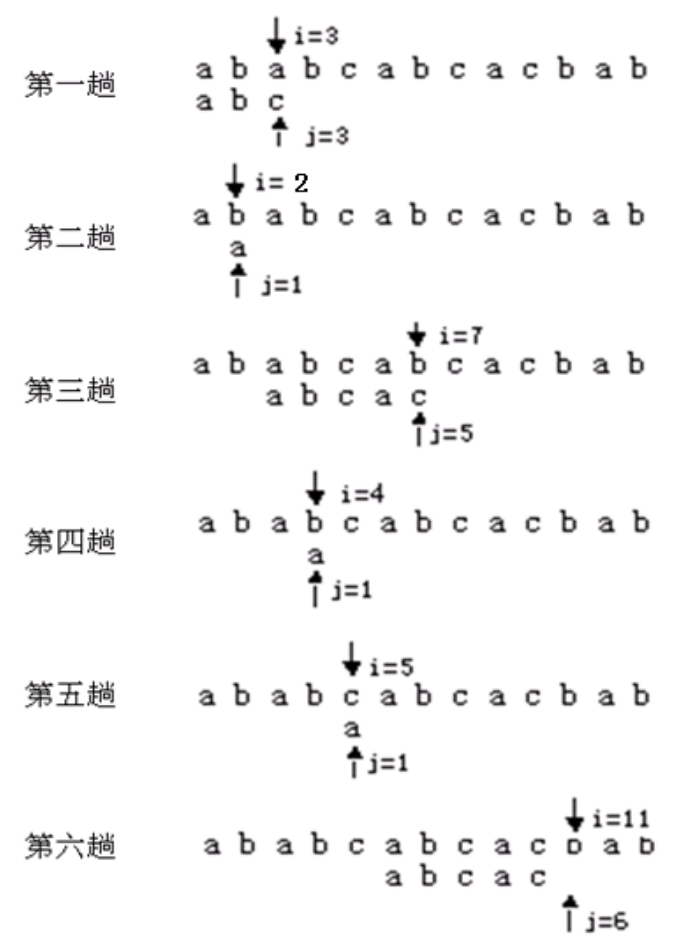
\includegraphics[width=0.9\textwidth]{figs/string/pattern-match.png}
    \end{column}
  \end{columns}
\end{frame}

\begin{frame}[fragile, allowframebreaks]
  \frametitle{Python示例代码}
  \small
  \begin{minted}{python}
def bf_search(source, target) -> tuple:
    """
    从source中查找出现的target,返回第一个位置的二元组
    主串中的位置, 比较次数),未找到返回(-1, 比较次数)
    """
    compare_count = 0
    for i in range(len(source)):
        found = True
        for j in range(len(target)):
            compare_count = compare_count + 1
            if source[i+j] != target[j]:
                found = False
                break
        if found:
            return i, compare_count
    return -1, compare_count

source = 'aaaaaaaaaaab'
target = 'aaaab'
position, compare_count = bf_search(source, target)

print('返回位置:', position)
print(f'在{source}的第{position}个位置开始,发现了{target},共比较了{compare_count}次')
print(source)
print('*'*position, end='')
print(target)
  \end{minted}

  \begin{minted}{text}
返回位置: 7
在aaaaaaaaaaab的第7个位置开始,发现了aaaab,共比较了40次
aaaaaaaaaaab
*******aaaab
  \end{minted}
\end{frame}


\begin{frame}[fragile]
  \frametitle{BF算法时间复杂度分析}
  \begin{itemize}
  \item 设串s长度为n,串t长度为m。匹配成功的情况下,考虑两种极端情况。
    \begin{itemize}
    \item 在最好情况下,即每趟不成功的匹配都发生在第一对字符比较时。
    \item 例如:s=“aaaaaaaaaabc”,t=“bc”,设匹配成功发生在$s_i$处。
    \item 在前面i-1趟不成功的匹配中共比较了i-1次,第i趟成功的匹配共比较了m次,所
      以总共比较了i-1+m次。
    \item 所有匹配成功的可能共有n-m+1种,设从si开始与t串匹配成功的概率为$p_i$,
      在等概率情况下$p_i=1/(n-m+1)$,因此最好情况下平均比较的次数是:
      \[\sum_{i=1}^{n-m+1} p_i \times (i-1+m) = \sum_{i=1}^{n-m+1} \dfrac{1}{n-m+1} \times (i-1+m) = \dfrac{(n+m)}{2}\]

    \item 即最好情况下的时间复杂度是$O(n+m)$
    \end{itemize}
  \end{itemize}
\end{frame}

\begin{frame}[fragile]
  \begin{itemize}
  \item 在最坏情况下,即每趟不成功的匹配都发生在t的最后一个字符。
  \item 例如:s=“aaaaaaaaaaab”,t=“aaab”,设匹配成功发生在$s_i$处.
  \item 在前面$i-1$趟匹配中共比较了$(i-1) \times m$次,第$i$趟成功的匹配共比较了
    $m$次,所以总共比较了$i \times m$次,因此最坏的情况下平均比较的次数是:
    \[\sum_{i=1}^{n-m+1} p_i \times (i \times m) = \sum_{i=1}^{n-m+1} \dfrac{1}{n-m+1} \times (i \times m) = \dfrac{m \times (n-m+2)}{2}\]
  \item 即最坏情况下的时间复杂度是$O(n×m)$
  \end{itemize}

  \begin{tcolorbox}[title=为什么BF算法时间性能低?]
    在每趟匹配不成功时存在大量回溯 (每次移动一位开始新的比较)
  \end{tcolorbox}
\end{frame}

\begin{frame}[fragile]
  \frametitle{改进算法}
  \scriptsize
  \begin{tikzpicture}[box/.style={draw, minimum width=0.6cm, minimum height=0.4cm}]
    \draw node[minimum width=2cm] (a0) {主串};
    \foreach \i in {1,...,7} {
      \pgfmathtruncatemacro{\x}{\i - 1};
      \draw node[box, right=0 of a\x] (a\i) {A} ;
    }

		\draw node[box, right=0 of a7] (a8) {B}  node[box, right=0 of a8] (a9) {A}  node[box, right=0 of a9] (a10) {A} ;

		\draw node[below=of a0] (b0) {子串}
		node[box, below=of a1] (b1) {A}
		node[box, below=of a2] (b2) {A}
		node[box, below=of a3] (b3) {A}
		node[box, below=of a4, fill=red!50] (b4) {B} ;

	  \draw[draw=red, very thick, <-] (a4) -- ++(0,1);
	  \draw[draw=red, very thick, <-] (b4) -- ++(0,-1);

    \path (a4) edge[draw=red, in=90, out=115, ->, dotted, thick]  (a2);
    \path (b4) edge[draw=red, in=-90, out=-115, ->, dotted, thick]  (b1);
  \end{tikzpicture}
  \small
  \begin{itemize}
  \item 改进算法的目的是在每一趟匹配过程中出现不匹配时,向右“滑动”尽可能远的一段
    距离后,继续进行比较。那么,应当滑动多远呢?这正是各个算法各显神通之处!

  \item KMP算法: 由D. E. Knuth,J. H. Morris和V. R. Pratt同时发现

    % \item Boyer-Moore算法
  \end{itemize}
\end{frame}

\begin{frame}[fragile]
  \frametitle{KMP算法}
  利用已经得到的“部分匹配”的结果将模式向右滑动

  视频讲解:
  \begin{itemize}
    \item \url{https://www.bilibili.com/video/BV1AY4y157yL/}
    \item \url{https://www.bilibili.com/video/BV1Er421K7kF/}
  \end{itemize}
\end{frame}

\begin{frame}[fragile]
  \frametitle{KMP算法}
  利用大语言模型来完成代码,已经变得非常方便,参见string.ipynb文件。

\end{frame}

\begin{frame}[fragile]
  \frametitle{练习}
  \begin{itemize}
  \item 从《红楼梦》中,统计主要人物出现的次数,并按照频次高低输出。

  \item 文件位置:ipynb/honglou.txt

  \item 人物列表:ipynb/honglou\_person.txt
  \end{itemize}
\end{frame}


\begin{frame}[fragile]
  \frametitle{多模式串匹配与AC自动机}
    \begin{itemize}
    \item BM、KMP为单模匹配,即模式串只有一个。假设主串$T[1, \cdots, m]$,
    模式串有k个$P={P_1,\cdots,P_k}$,且模式串集合的总长度为$n$。
    如果采用KMP来匹配多模式串,则算法复杂度为:

    \[O(|P_1|+m+\cdots+|P_k|+m)=O(n+km)\]
  
    \item KMP并没有利用到模式串之间的重复字符结构信息,每一次模式串的匹配都需要将主串从头至尾扫描一遍。

    \item 贝尔实验室的Aho与Corasick于1975年基于有限状态机(finite state machines)提出AC自动机算法
  \footnote{AC算法比KMP提出要早,KMP于1977年提出}。
  \end{itemize}
  % https://www.cnblogs.com/en-heng/p/5247903.html
\end{frame}

\begin{frame}[fragile]
  \frametitle{AC自动机}
  \begin{itemize}
  \item 自动机由状态(数字标记的圆圈)和转换(带标签的箭头)组成,每一次转换对应一个字符。AC算法的核心包括三个函数:goto、failure、output;这三个函数构成了AC自动机。对于模式串{he, his, hers, she},goto函数表示字符按模式串的转移,暗含了模式串的共同前缀的字符结构信息\footnote{\url{from: https://www.cnblogs.com/en-heng/p/5247903.html}}。
  \end{itemize}

  \begin{center}
  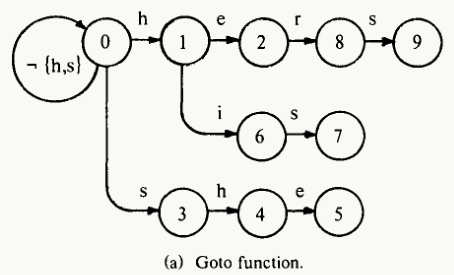
\includegraphics[width=0.55\textwidth]{figs/string/ac_goto.png}
  \end{center}
\end{frame}

\begin{frame}[fragile]
  \frametitle{AC自动机}
  \begin{itemize}
  \item failure函数表示匹配失败时退回的状态:
  \end{itemize}

  \begin{center}
  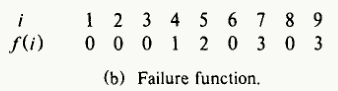
\includegraphics[width=0.6\textwidth]{figs/string/ac_failure.png}
  \end{center}
\end{frame}

\begin{frame}[fragile]
  \frametitle{AC自动机}
  \begin{itemize}
  \item output函数表示模式串对应于自动机的状态:
  \end{itemize}

  \begin{center}
  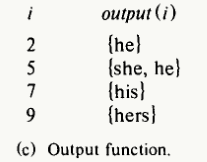
\includegraphics[width=0.4\textwidth]{figs/string/ac_output.png}
  \end{center}
\end{frame}

\begin{frame}[fragile]
  \frametitle{AC自动机}
  \begin{itemize}
  \item 完整的AC自动机如下:
  \end{itemize}

  \begin{center}
  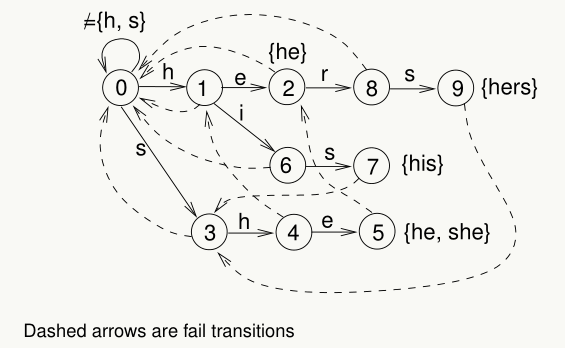
\includegraphics[width=0.8\textwidth]{figs/string/ac.png}
  \end{center}
\end{frame}

\begin{frame}[fragile]
  \frametitle{AC自动机匹配过程}
  AC算法根据自动机匹配模式串,过程比较简单:从主串的首字符、自动机的初始状态0开始,

  \begin{itemize}
  \item 若字符匹配成功,则按自动机的goto函数转移到下一状态;且若转移的状态对应有output函数,则输出已匹配上的模式串;
  \item 若字符匹配失败,则递归地按自动机的failure函数进行转移
  \end{itemize}
\end{frame}


\begin{frame}[fragile]
  \frametitle{Python实现:pyahocorasick}
  \begin{itemize}
  \item \url{https://pypi.org/project/pyahocorasick/}
  \item \url{https://www.bilibili.com/video/BV1yA4y1Z74t/}
  \end{itemize}
\end{frame}